\documentclass{beamer}
\usetheme{default}
\setbeamertemplate{footline}[frame number]
\title{Bringing Expectations to the Collective Bargaining Table}
\subtitle{Evidence From Brazilian Firms}
\date{\today}
\usepackage{booktabs}
\begin{document}
\begin{frame}
\titlepage
\end{frame}


\begin{frame}
\frametitle{Outline}
\tableofcontents
\end{frame}

\section{Introduction}
\begin{frame}
\frametitle{Main Questions}
	\begin{itemize}
		\item How do inflationary news shocks affect collective bargaining outcomes (wages and employment)?
		\item How does the timing of collective bargaining agreements (CBAs) affect firm performance?
		\item What are the macroeconomic implications of collective bargaining activity induced by inflationary news shocks? 
	\end{itemize}
\end{frame}

\begin{frame}
\frametitle{Economic Significance}
	\begin{itemize}
		\item Inflation expectations and economic behavior
		\item Monetary policy application: forward guidance
			\begin{itemize}
				\item Traditional channels are consumption and investment. Analyze potential CBA channel
			\end{itemize}
		\item Timing of monetary policy Shocks (Tenreyro \& Olivei 2007 AER)
		\item Nominal rigidity \--- wage adjustment asymmetries (Kaur 2019 AER)
	\end{itemize}
\end{frame}

\section{Data}
\begin{frame}
\frametitle{Data}
	\begin{itemize}
		\item RAIS \--- Matched employer-employee data 
		\item Sistemas Mediador \--- collective bargaining agreements (single firm - employee contracts)
		\item IBRE / IBGE \--- aggregate inflation expectations	(May gain access to firm-level price and cost expectations)
	\end{itemize}
\end{frame}

\begin{frame}
\frametitle{Background}
	\begin{itemize}
		\item Dual economic and political crises in Brazil 2015 - 2016
		\item  Impeachment of President Dilma Rousseff announced on December 2, 2015. Her powers were suspended on May 12, 2016.
		\item \textbf{Inflationary news shock:} In June 2016, acting President Michel Temer appointed Ilan Goldfajn as the BCB head.
		\centering
		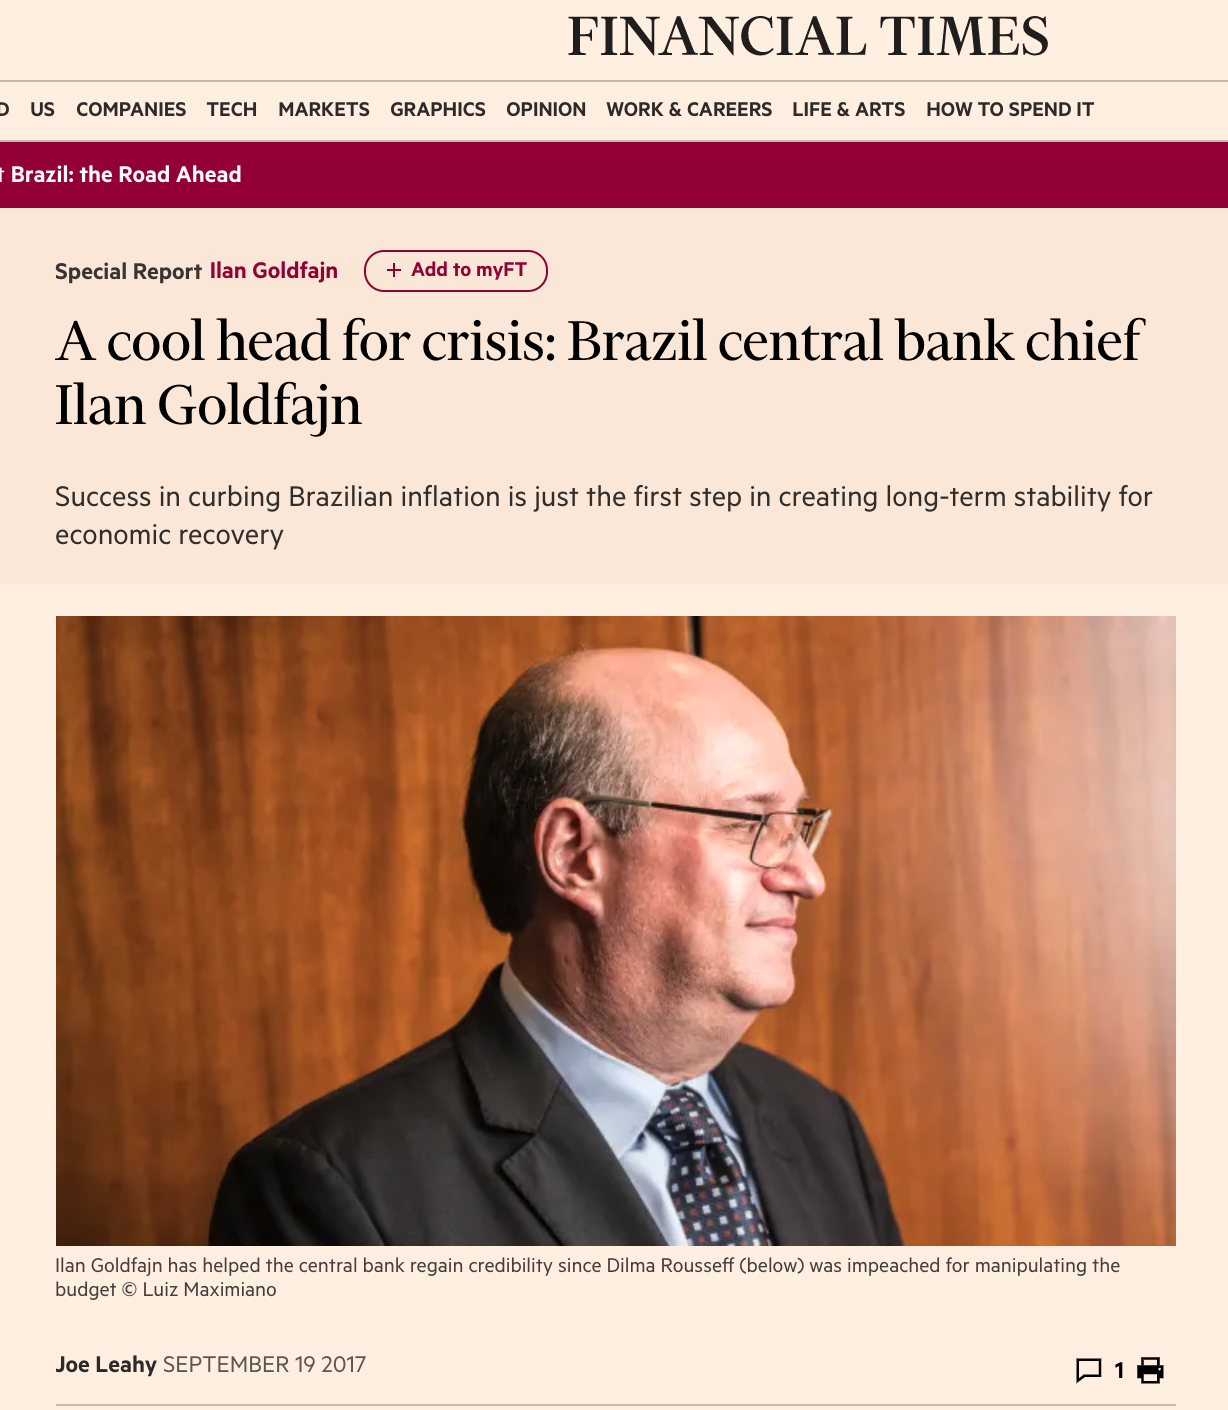
\includegraphics[scale=.2]{old_figures/goldfajn.png}
	\end{itemize}
\end{frame}

\section{Preliminary Findings}
\begin{frame}
\frametitle{Preliminary Findings}
	\begin{itemize}
	\item Across all sectors, inflation expectations rose to 12\% until February 2016, at which point they began to decline to roughly 5\% by Q3 2017 (as anticipation of new regime took root.)
	\item Timing of CBAs provides opportune variation for studying effects on wages, employment
	\item Setting may allow us to analyze multiple inflation shocks prior to 2017
	\end{itemize}
\end{frame} 
\begin{frame}
		\centering
		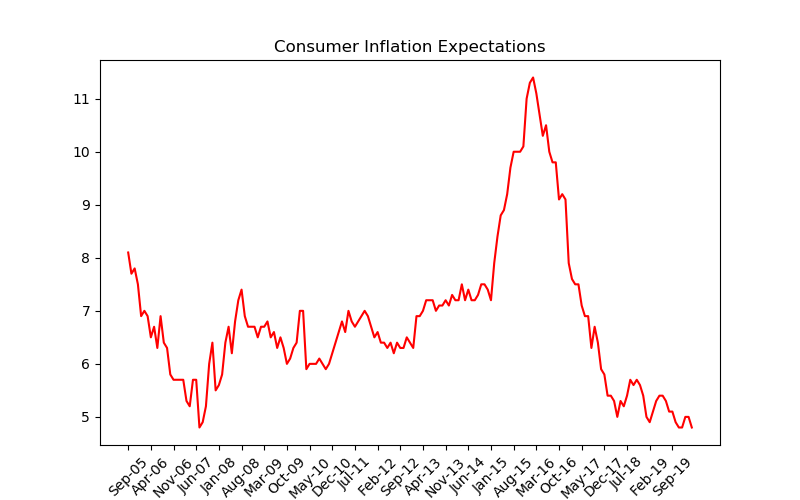
\includegraphics[scale=.6]{old_figures/IBRE_Consumer_Inflation_Expectations.png}
\end{frame}


\begin{frame}
		\centering
		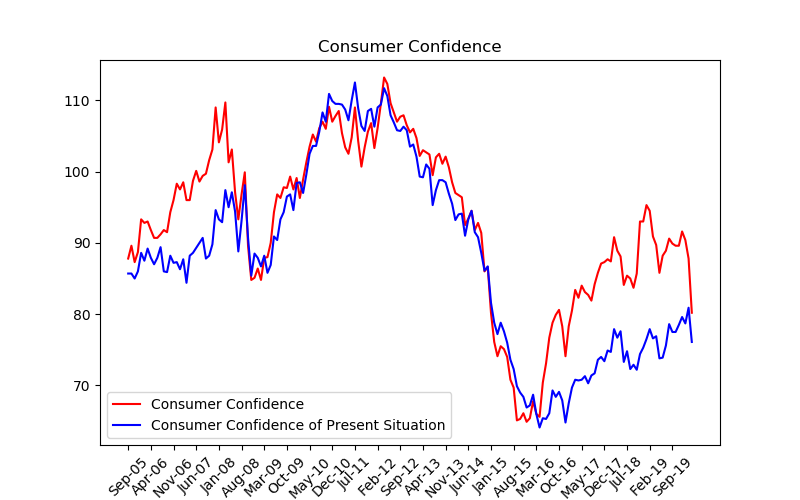
\includegraphics[scale=.6]{old_figures/IBRE_Consumer_Expectations}
\end{frame}

\begin{frame}
		\centering
		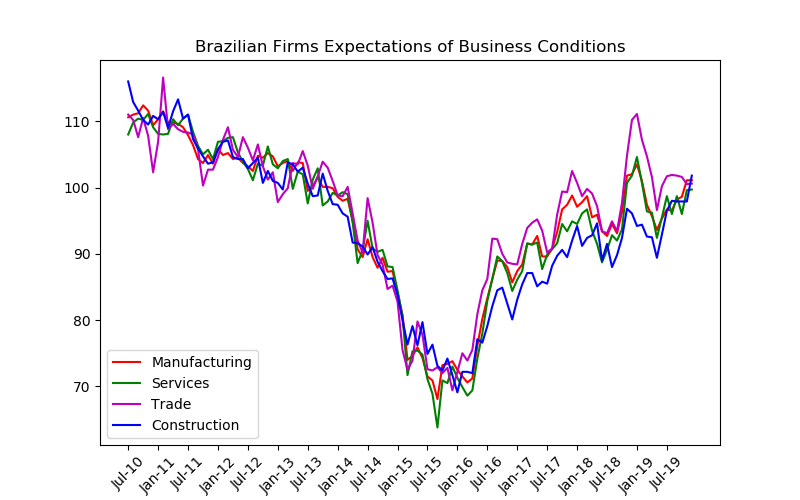
\includegraphics[scale=.6]{old_figures/IBRE_Firm_Expectations}
\end{frame}

\begin{frame}
\frametitle{Actual Inflation in Brazil}
	\centering
	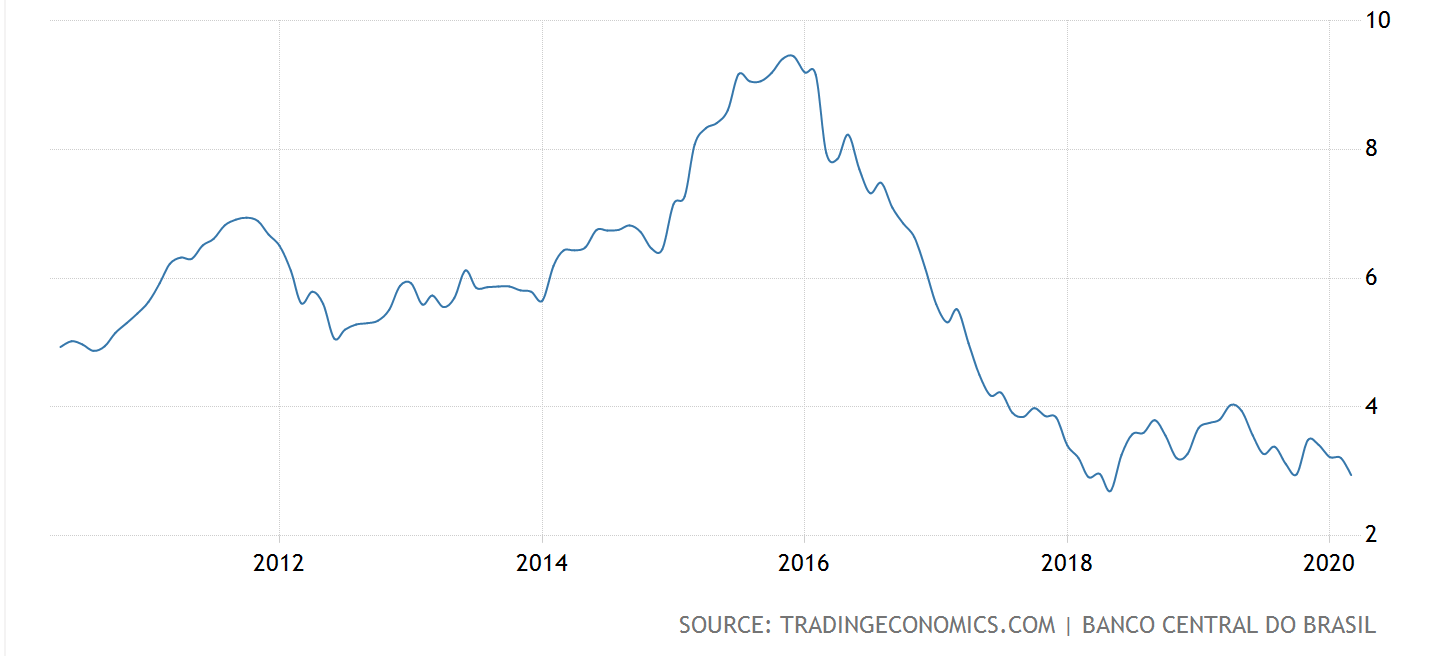
\includegraphics[scale=.45]{old_figures/Brazil_Inflation.png}
\end{frame}

\begin{frame}
\frametitle{Average Monthly Real Wages in Brazil}
	\centering
	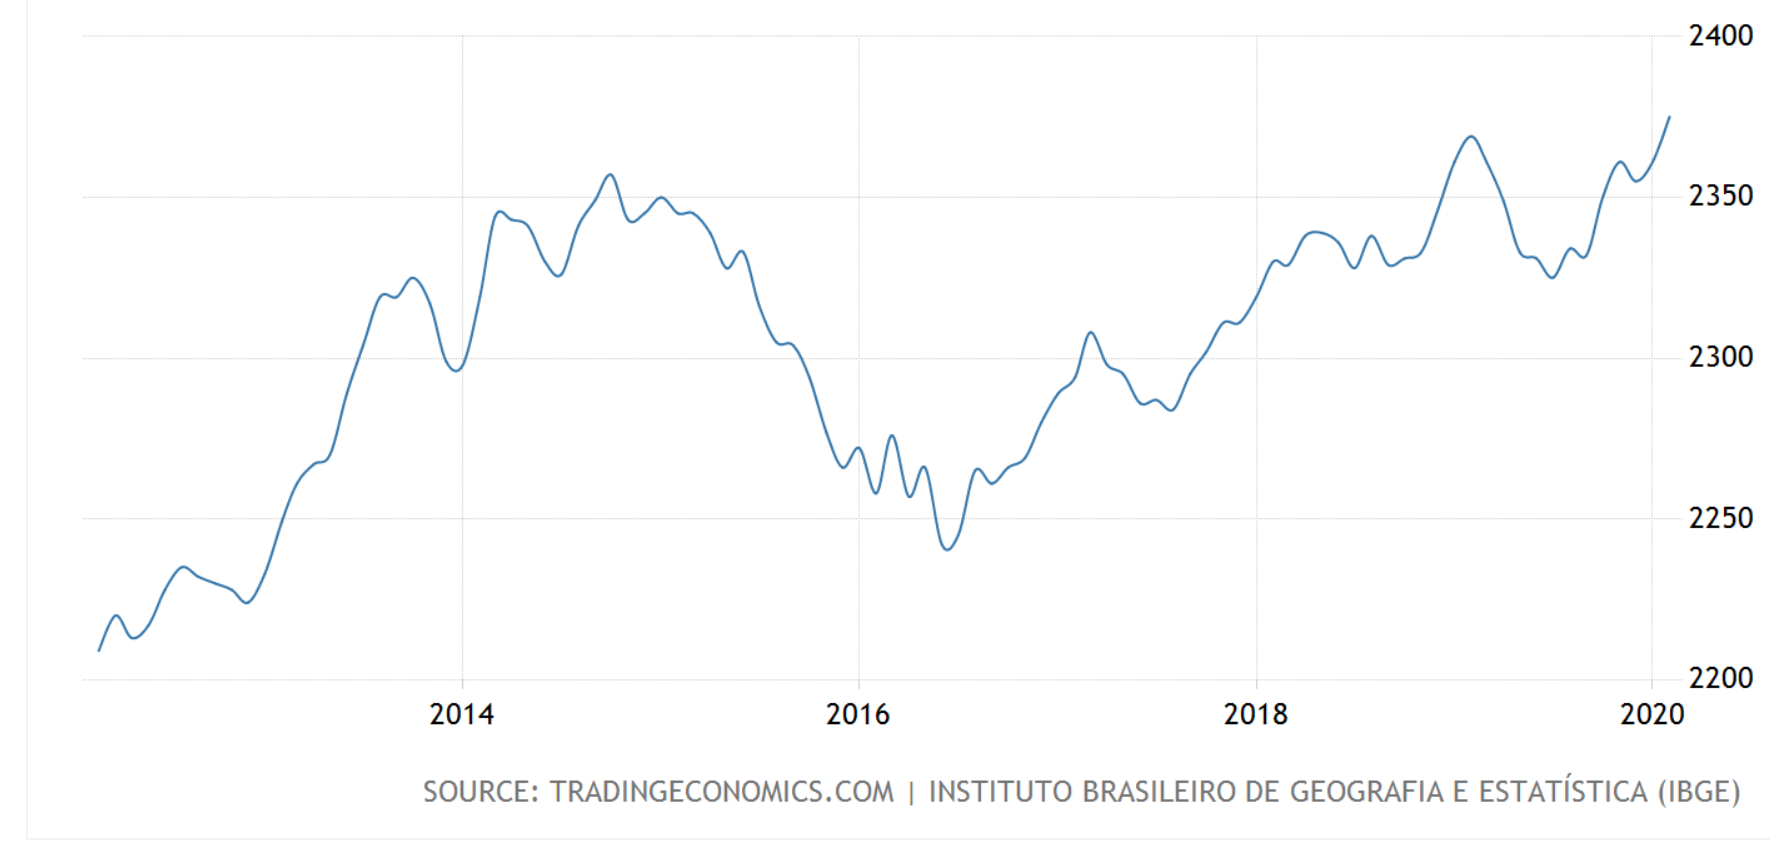
\includegraphics[scale=.35]{old_figures/Wage_Growth.png}
\end{frame}

\begin{frame}
\frametitle{Timing of CBAs in Brazil}
		\begin{center}
		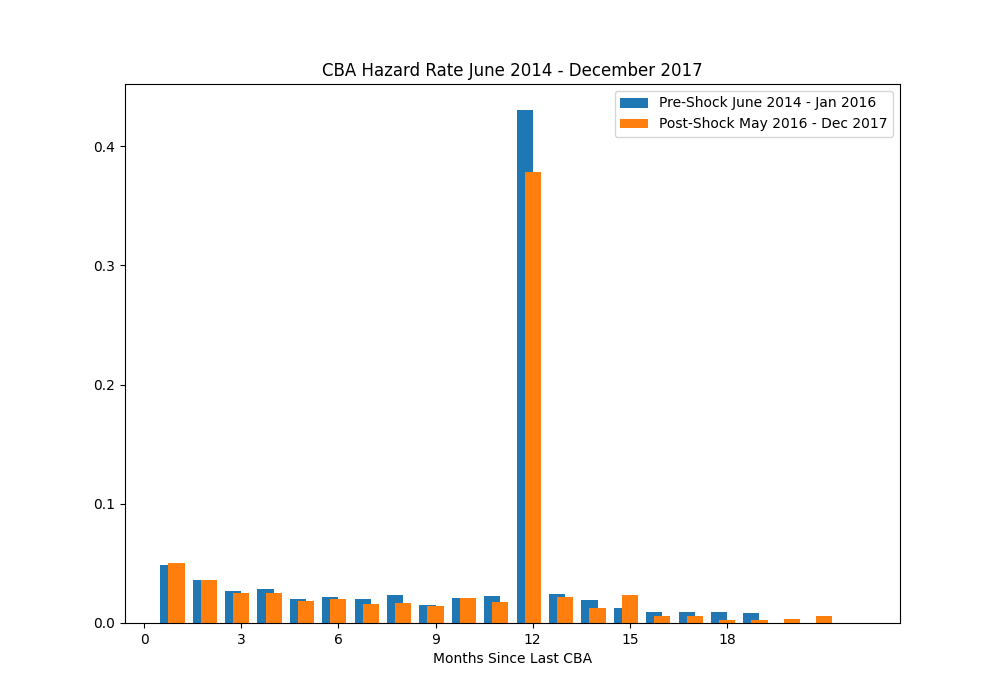
\includegraphics[scale=.45]{tables-figures/cba_hazard.png}
		\end{center}
\end{frame}

\begin{frame}
\frametitle{Timing of CBAs in Brazil}
		\centering
		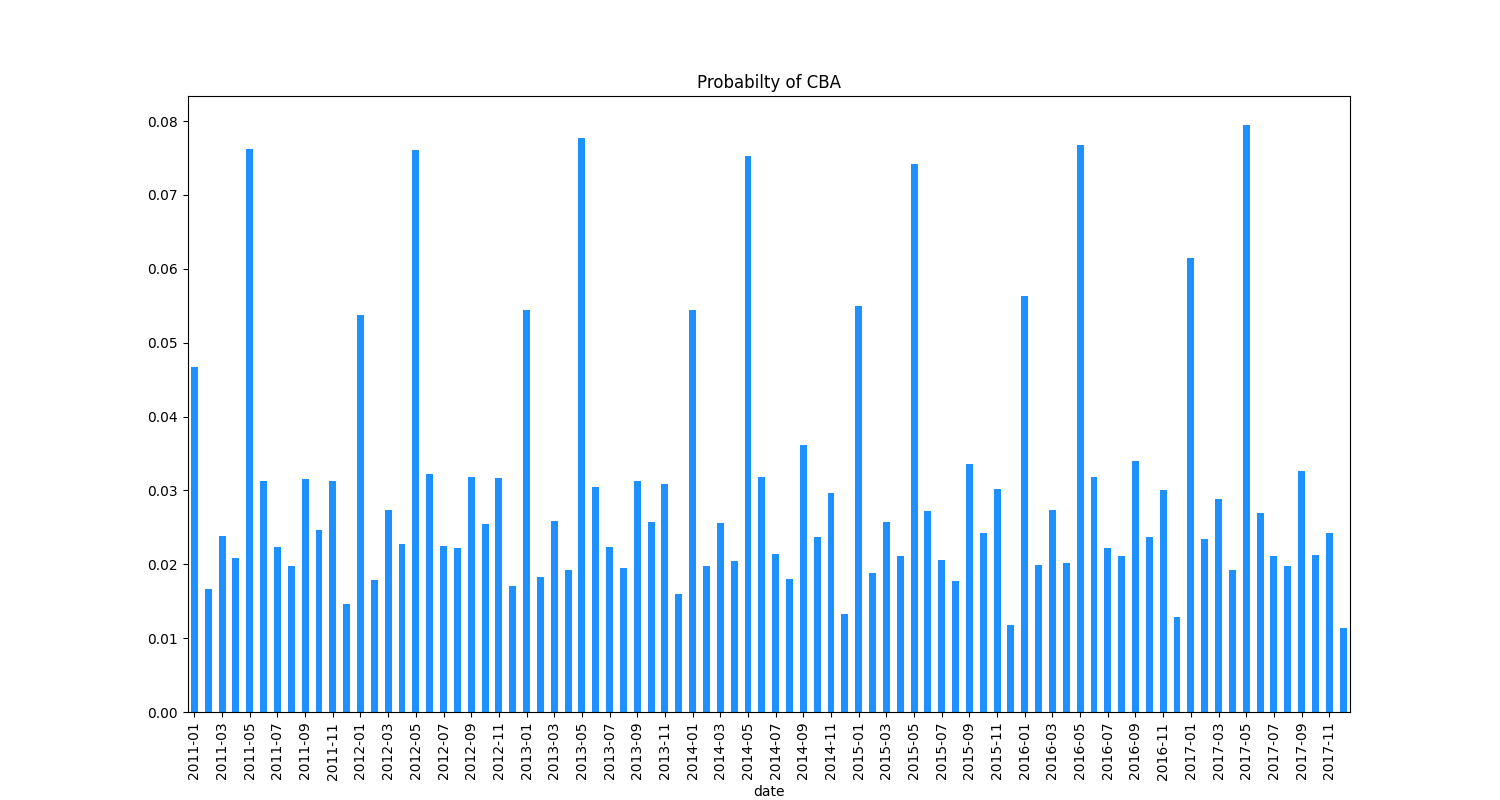
\includegraphics[scale=.3]{tables-figures/cba_probability.png}
\end{frame}

\begin{frame}
	\frametitle{Reduced-Form Model 1}
	We focus on the subset of firms with a one-year contract set either in Jan 2016 (pre-shock) or Mar 2016 (post-shock). Using a DiD approach, we measure the effect on nominal wage growth of setting wages just before the shock and just after:
	\begin{align*}
		nom\:wage_{i,t} = \beta_0 + \beta_1 D_{t}^{March\:2016} + \beta_2 D^{March\:CBA}_{i} +\\
		 \beta_3[ D_{t}^{March\:2016} \times D^{March\:CBA}_{i}] + \mathbf{Z}_{i,t} + \varepsilon_{i,t}
 	\end{align*}
 	\begin{itemize}
 		\item $\beta_3$ captures the difference in nominal wage differences across firms with pre- and post- shock CBAs
 		\item Caveat: nominal wage growth may be driven by other forms of negotiation, even if a firm is ``locked-into''  a CBA
 	\end{itemize}
\end{frame}
\begin{frame}
	\frametitle{Reduced-Form Model 2}
		A preliminary reduced-form model takes the following form:
		\begin{align*}
			nominal\_wage\_growth_{i,t} & = \alpha + \beta_1 exp\_inflation_t \times CBA\_month_{i,t} +\\
			& \beta_2 CBA\_month_{i,t} + \beta_3 exp\_inflation_t + \mathbf{Z_{i,t}} + \varepsilon_{i,t} 	
		\end{align*}
\end{frame}


\begin{frame}
	\begin{center}
			\scalebox{.45}{{
\def\sym#1{\ifmmode^{#1}\else\(^{#1}\)\fi}
\begin{tabular}{l*{3}{c}}
\hline\hline
            &\multicolumn{1}{c}{(1)}         &\multicolumn{1}{c}{(2)}         &\multicolumn{1}{c}{(3)}         \\
\hline
inflation\_CBA\_interaction&       1.853\sym{***}&                     &       0.600\sym{***}\\
            &     (0.365)         &                     &    (0.0946)         \\
lag1\_inflation\_CBA\_interaction&      -1.313\sym{***}&       0.518\sym{***}&                     \\
            &     (0.383)         &    (0.0992)         &                     \\
cba\_month   &     -0.0214\sym{**} &     -0.0208\sym{**} &     -0.0275\sym{***}\\
            &   (0.00801)         &   (0.00802)         &   (0.00768)         \\
exp\_inflation&      -0.978\sym{***}&                     &      -1.528\sym{***}\\
            &    (0.0549)         &                     &   (0.00966)         \\
lag1\_exp\_inflation&      -0.577\sym{***}&      -1.553\sym{***}&                     \\
            &    (0.0567)         &    (0.0100)         &                     \\
m2          &      0.0946\sym{***}&      0.0917\sym{***}&      0.0966\sym{***}\\
            &   (0.00167)         &   (0.00164)         &   (0.00166)         \\
m3          &       0.156\sym{***}&       0.154\sym{***}&       0.157\sym{***}\\
            &   (0.00155)         &   (0.00153)         &   (0.00154)         \\
m4          &       0.129\sym{***}&       0.127\sym{***}&       0.131\sym{***}\\
            &   (0.00144)         &   (0.00141)         &   (0.00143)         \\
m5          &       0.159\sym{***}&       0.159\sym{***}&       0.158\sym{***}\\
            &   (0.00149)         &   (0.00149)         &   (0.00149)         \\
m6          &       0.134\sym{***}&       0.130\sym{***}&       0.136\sym{***}\\
            &   (0.00146)         &   (0.00144)         &   (0.00146)         \\
m7          &       0.162\sym{***}&       0.160\sym{***}&       0.163\sym{***}\\
            &   (0.00150)         &   (0.00148)         &   (0.00149)         \\
m8          &       0.132\sym{***}&       0.131\sym{***}&       0.133\sym{***}\\
            &   (0.00145)         &   (0.00144)         &   (0.00145)         \\
m9          &       0.129\sym{***}&       0.126\sym{***}&       0.131\sym{***}\\
            &   (0.00139)         &   (0.00138)         &   (0.00140)         \\
m10         &       0.157\sym{***}&       0.157\sym{***}&       0.157\sym{***}\\
            &   (0.00147)         &   (0.00147)         &   (0.00147)         \\
m11         &       0.132\sym{***}&       0.130\sym{***}&       0.133\sym{***}\\
            &   (0.00139)         &   (0.00138)         &   (0.00139)         \\
m12         &       0.353\sym{***}&       0.349\sym{***}&       0.355\sym{***}\\
            &   (0.00236)         &   (0.00233)         &   (0.00236)         \\
\_cons      &    -0.00626\sym{***}&    -0.00449\sym{***}&    -0.00990\sym{***}\\
            &  (0.000978)         &  (0.000946)         &  (0.000926)         \\
\hline
\(N\)       &     5462768         &     5462768         &     5462768         \\
\hline\hline
\multicolumn{4}{l}{\footnotesize Standard errors in parentheses}\\
\multicolumn{4}{l}{\footnotesize \sym{*} \(p<0.05\), \sym{**} \(p<0.01\), \sym{***} \(p<0.001\)}\\
\end{tabular}
}
}
	\end{center}
\end{frame}

\begin{frame}
\frametitle{Structural Identification Strategy}
	\begin{itemize}
		\item Adapt a staggered wage model with collective bargaining to assess impacts of monetary policy  
		\item Estimate effects on economy-wide wages, levels of employment
	\end{itemize}
\end{frame}
\end{document}
